\chapter{Hardware}
% ------------------------

\section{Hardware Overview}
% Joey (get started)

The hardware part consists of two main blocks: NIOS System on Programmable Controller and the Tester.

\begin{figure}
 \centering
 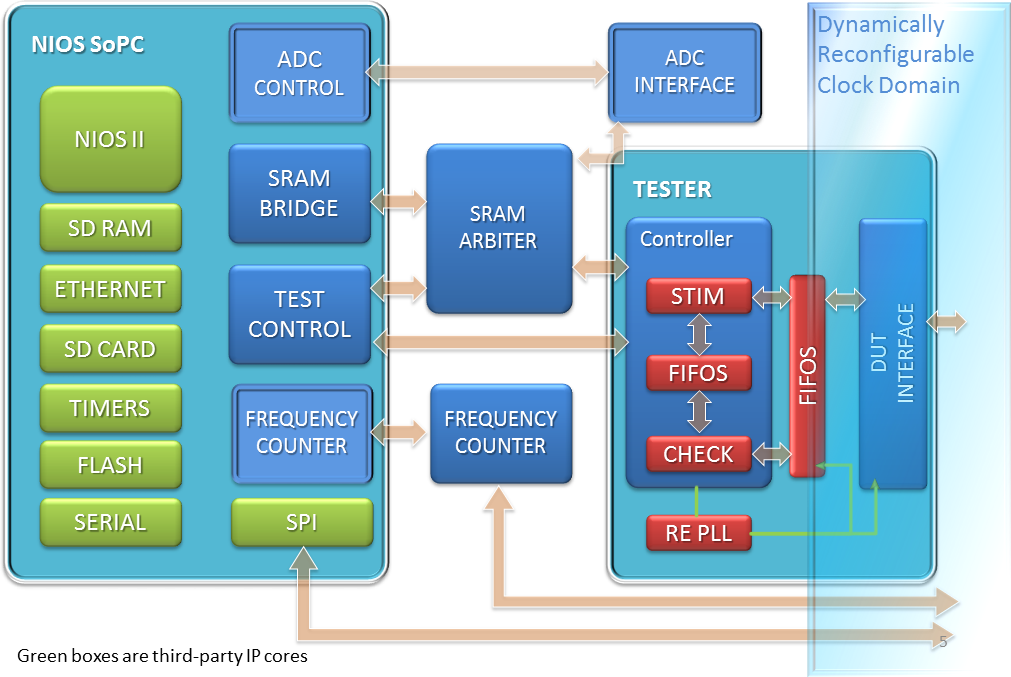
\includegraphics[width=0.9\textwidth]{hw_overview}
 \caption{Hardware Overview.}
 \label{fig:hw_overview}
\end{figure}



The \textit{NIOS SoPC} coordinates the whole system, writing the data from SD Card into the SRAM for the Tester to read the data from it; retrieving the result that the Tester writes back to the SRAM and sending the data to the backend for archiving and reviewing for the users. Its tasks include:
\begin{itemize}
 \item coordinate the data from multiple sources (SRAM, SD Card, Flash, Serial connection, SPI bus, Ethernet, etc.)
 \item control the testing process (which is executed by the Tester, frequency counter and ADC)
 \item send results to the backend
 \item user interface
\end{itemize}

The \textit{SRAM arbiter} is the interface between the SoPC, tester and the SRAM by Avalon Memory Mapped Interface (Avalon-MM). It handles the SRAM read and write requests from SoPC and tester.

The \textit{Tester} contains several HDL blocks which are responsible for the testing process.
\begin{itemize}
 \item read the command, request and test vector from SRAM
 \item generate the test input signals for every pin of the DUT
 \item monitor the output pins of the DUT and write the result into the memory when the it is valid
 \item offer a dynamically reconfigurable clock for the DUT and its relative interface
\end{itemize}

The purpose of the \textit{frequency counter} and the \textit{ADC} is that there is a designated pin on the chip which is the output of a ring oscillator. It is preferable that not only the frequency of this clock output is tested, but that the output waveform is also monitored.


\section{PCB (interface board)}
% Nano (and Joey)

For the chip tester, two PCBs are needed in this project. One which is called $B2$ has been designed for the virtual designs to be loaded in a slave FPGA. The other is called $B1$ that is developed as an interface for those real chips are about to be tested. Both PCBs are two layers board and designed by using Allegro $16.3$ PCB designer tools. The dimensions of $B1$ and $B2$ are $98.93 mm* 68.5 mm$ and $81.28 mm * 68.33 mm$ and the minimum wire size is $8mm$.

\subsection{B1 (DUT testing board)}

\subsubsection{DUT}

The superchip under test has the following specific features:
\begin{itemize}
 \item $6$ separate design sites
 \item $24$ digital input pins [$A0\dots A23$], shared between all design sites;
 \item $4$ digital output pins [$Q0\dots Q23$], shared between all design sites;
 \item $16$ separate VDD pins, one dedicated to each design site;
 \item $1$ global GND pin for all design sites and infrastructure circuitry;
 \item $1$ global VDD pin to power the site buffers and I/O pad ring;
 \item $68$-pin JLCC package (with 2 unused pins).
\end{itemize}

The chip is interfaced with the PCB by a 68WAY PLCC socket. The power is supplied by the $3.3V$ VDD from the DE2 board. The GND is also connected to the DE2 GND.

The shared I/Os are connected to the powered design site, and disconnected from the other design sites. Hence a controllable power switch is designed with a 4-16 decoder and an integrated power switch array. The $Q1$ is the output of a ring oscillator. The frequency can be digitally tested by the general I/O. However, to examine the analog properties of this output, an analog part including a buffer, $3^{rd}$ order Butterworth filter and ADC with their own power supply is also designed.


\subsubsection{Digital Part}

\paragraph{Decoder}
Although there are 16 design sites to be selected, the data can be shrunk down to $4$ bits to save space of the test vector and metadata, since only one site is selected at a time. The decoder we used is $74HC4514$, a $4-to-16$ line decoder with latch. The input and output are active high.

\paragraph{Switch Array}
The switch array consists of four $TPS2095$ quad power-distribution switches. One could simply use a CMOS to realize a switch. However, with thermal sense, current limit and charge pump, the $TPS2095$ switches are more reliable, stable, smooth (minimum switching current surges) and relatively compact in scale. The operation of a switch is simple: when EN pin is asserted, the OUT pin offers the power with the same voltage in the IN pin. Otherwise the OUT pin is disconnected from the input power. In one $TPS2095$ chip there are 4 such switches, the EN pins of which are all active high.


\subsubsection{Analog Part}

\begin{figure}
 \centering
 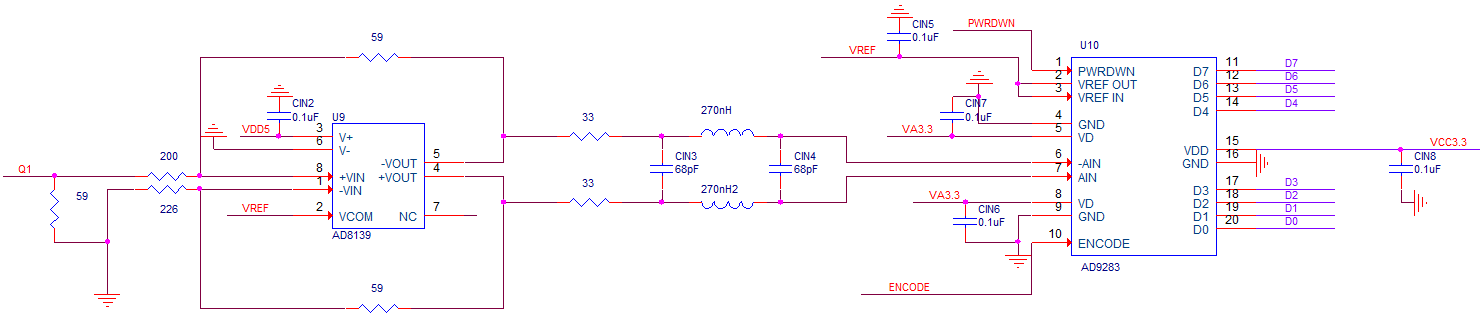
\includegraphics[width=0.95\textwidth]{analog_1}
 \caption{Analog Part Overview.}
 \label{fig:analog_overview}
\end{figure}

\paragraph{Buffer}
An $AD8139$ differential ADC driver is used as the front buffer of the ADC. It is an ultralow noise, high performance differential amplifier with rail to rail output from Analog Devices. The designed gain of the buffer is $0.295$, and the differential gain is approximately $0.14$.

\paragraph{ADC}
The $8-bit$, $100MSPS$ ADC is used to convert the analog signal. The encode clock is the clock from the DE2 board ($100MHz$ by default). A power-down function select is also connected to the FPGA for shutting down the ADC when it’s not in use. The ADC signal wires should be placed far away from the other wires for minimum interference; and they should also be placed parallel to each other to have similar length for better signal integrity. However, since the pin density is too high of the HSMC connector we used, it is inevitable that the ADC wires are closed to the other wires. The ADC is placed on the other side of the PCB board for a better result.

\paragraph{Butterworth Filter}
To minimize the high frequency noise, a third-order low pass Butterworth filter is designed. With three poles, the attenuation is $-60 \sfrac{dB}{decade}$ on signals higher than the cut-off frequency. The filter topology used here is balanced ladder topology. Automatic design tool Elsie is used for designing the parameters of the RCI circuit. The cut-off frequency is $40MHz$.

\paragraph{Separate Power Supplies}
The buffer and ADC are separately powered from the other parts of the board. The $AD8139$’s power ranges from $5V$ to $12V$, and the ADC ranges from $2.7V$ to $3.6V$. Two low dropout regulators (LDP), $ADP3335$ and $ADP3333$ are used to offer $5V$ and $3.3V$ voltages respectively. The supply voltage of these two LDP ranges from $2.6V$ to $12V$. Their load currents are up to $500mA$ and $300mA$ respectively.

\subsection{B2 (Virtual design board)}

\subsubsection{Slave FPGA}

Slave FPGA is the core chip of the virtual design board. It can be used for programing designs when they are going to be tested. An Altera Cyclone III FPGA will be implemented as the slave FPGA.

Cyclone III ($EP3C25E144$) belongs to Cyclone III device family. With densities ranging from about $5,000$ to $200,000$ logic elements (LEs) and $0.5Mb$ to $8Mb$ of memory for less than $\sfrac{1}{4}V$ of static power consumption, Cyclone III devices makes it easier to meet the power budget \citep{Altera:2011:cyclone3handbook}.

The reason for choosing Cyclone III is their lowest power, high functionality with the lowest cost. $144$ pins are enough for this design. I/O pins on the Cyclone III are grouped together into I/O banks, and each bank has a separate power bus. There are eight I/O banks, as shown in \hl{Figure 1} \citep{Altera:2011:cyclone3handbook}. All single-ended I/O standards are supported in all banks except HSTL-12 Class II which is only supported in column banks. The same case can be found in all differential I/O standards.


Each I/O banks of Cyclone III has a VREF bus to accommodate voltage-referenced I/O standards. Connect the VREF pin of each group to the appropriate voltage. In this design three voltage levels, which $VCCIO=3.3V$, $VCCINT= 1.2V$ and $VCCA=2.5V$, are necessary. Proper bypassing and decoupling technique for the power pins is very important for reliable design operation. In this case, additional decoupling capacitance is needed. The VCCINT, VCCIO and ground pins should add as many as $0.2\mu F$ power-supply decoupling capacitors as possible. So $0.01 \mu F$ capacitor for VCCIO and $0.1 \mu F$ for VCCINT seems to be appropriate. Note that all the capacitors should be place close enough to the power pins.

In regard of the Cyclone III configuration, the Cyclone II device uses SRAM cells to store configuration data. $EP3C25E144$ can only be configured in Fast Active serial (AS) mode.

Configuration data is loaded into Cyclone III at each DCLK cycle. As soon as the device receives all data, the device releases the open-drain CONF\_DONE pin, which is pulled high by an external 10- pull-up resistor. The CONF\_DONE pin transits low-to-high to indicate that configuration is complete and initialization of the device can begin. The CONF\_DONE pin must have a 10- pull-up resistor for initialization.

Pulling the nCONFIG pin low can begin reconfiguration and this pin must be low for at least $500ns$. The Cyclone III device is reset when nCONFIG is pulled low. Meanwhile, the device will pulls nSTATUS and CONF\_DONE low and I/O pins are tri-stated. When nCONFIG returns to high and nSTATUS is released, reconfiguration begins.

The clock source for initialization is either a $10MHz$ (typical) internal oscillator or an optional CLK pin. In this situation, an external oscillator (A $TXC-50MHz$ oscillator is going to be introduced later) will be implemented as the clock source. The required clock for initialization in Cyclone III is $3,185$ and the maximum CLK frequency is $133MHz$.

The configuration mode is selected by driving the MSEL pins either low or high. The MSEL pins can be powered by VCCIO and GND. For AS mode, MSEL [1] should be pulled up by connecting to VCCIO. MSEL [0] and MSEL [2] are pulled down by connecting to GND. The MSEL pins have $9$ internal pull-down resistors that are always active.

The maximum active master frequency for Cyclone III is $30MHz$ typically and device only work with serial configuration devices that support up to $40MHz$.

In AS mode, Cyclone III reads the configuration data providing by serial configuration (A Spansion SPI Flash is going to be introduced later) via a serial interface. The serial configuration device controls the configuration interface.

There are four pins on the serial configuration devices:
\begin{itemize}
 \item Serial clock input (DCLK)
 \item serial data output (DATA)
 \item As data output (ASDI)
 \item Active-low chip select (nCS)
\end{itemize}

Connect these four pins to Cyclone III device pins, as shown in \hl{Figure 2.}


A $25\Omega$ series resistor must connect a between serial configuration device and the Cyclone III device at the near end of the serial configuration device for DATA [0] when configure the Cyclone III device in the AS mode. The $25\Omega$ resistor works to minimize the driver impedance mismatch with the board trace and reduce the overshoot seen at the Cyclone III device input pin DATA [0].

The maximum trace length between Cyclone III device and the serial configuration device, in another words, the CLK, DATA [0], NCSO and ADSO pins, must less than $10in$. In the B1 PCB designing, only $8mm$ is used.

Cyclone III device uses a $40MHz$ internal oscillator to generate DCLK to controls the entire configuration cycle and provide timing for the serial interface.

By driving the nCSO output pin low, which connect to nCS pin of the configuration device, the Cyclone III device enables the configuration device.  DCLK and DATA [1] pins are used to send operation commands and read address signals to the serial configuration device. The configuration device sends data on DATA pin which connects to the DATA [0] pin of the Cyclone III device. After all the configuration bits are received, cyclone III releases the open-drain CONF\_DONE pin with a $10\Omega$ pull-up resistor. The CONF\_DONE pin must have an external $10\Omega$ resistor for the device to initialize.





\subsubsection{Serial Configuration Device}

Cyclone III FPGAs are programmable logic devices used for basic logic functions, chip-to-chip connectivity, signal processing, and embedded processing. They can be programmed and configured by a microprocessor, JTAG port, or directly bay a serial PROM or flash. Spansion SPI (Serial Peripheral Interface) flash $S25FL064K$ can configure the FPGA easily at power-up \citep{Spansion:2011:appnote}.

The three stages of the configuration cycle are power-on reset, configuration, and initialization. When the FPGA enters power-on rest (POR), it drives the nSTATUS signal low to indicate it is busy, drives the CONF\_DONE signal low to indicate the configuration has not been completed, and tri-states all I/O pins. All pins will be released after POR.

The DCLK generated by the FPGA device control the configuration data transferring. The CONF\_DONE pin will be released with pulling high by an external pull-up resistor after all configuration data is transferred to the FPGA. The FPGA enters user mode after internal initialization.

The SPI is a simple four-pin synchronous interface protocol which enables a master device and one or more slave devices to intercommunicate. Four signal wires are:
\begin{itemize}
 \item Master Out Slave In (MOSI) signal generated by the master (data to slave)
 \item Master In Slave Out (MISO) signal generated by the slave (data to master)
 \item Serial Clock (SCK) signal generated by the master to synchronize data transfers
 \item Slave Select (SS) signal generated by master to select individual slave devices (also known as Chip Select (CS) or Chip Enable (CE))
\end{itemize}


\hl{Figure 3} displays a simple block diagram of the connection between FPGA and SPI flash, as well as the HSMC header and JTAG programming the SPI flash from a host PC.


\hl{Figure 4} displays the details of the connection between SPI flash and FPGA. According to the introduction of Cyclone III, we can acquire the whole routing of FPGA, SPI flash and the HSMC header (A Samtec ASP header will be introduced later).



The TMS, TDI, TDO and TCK pins of Cyclone III device are used to operating in the IEEE Std. 1149.1 BST. The TDO pin is powered by VCCIO (3.3V). TDI and TMS are powered by VCCA (2.5V).

The header for JTAG and the header for SPI Flash In-system is use the same HSMC header with 172 pins which is quite enough for these two headers.





\subsubsection{External Oscillator}

As mentioned in the Cyclone III part, an external oscillator is needed as the clock source to provide certain frequency for the FPGA. A $50MHz$ oscillator of TXC will be implemented. The typical clock frequency for Cyclone III device is $30HMz$ and the maximum is $40MHz$. The TXC DEL04 oscillator is a sealed clock crystal oscillator unit with high precision characteristic covering up to wide frequency range ($1MHz$ to $170 MHz$), which is appropriate for the FPGA. The supply voltage range is $1.8V \sim 5V$ \citep{TXC:osc_datasheet}.



\subsubsection{Voltage Regulator}

The $B2$ board needs at least three different voltage levels, as mentioned before, $VCCIO=3.3V$, $VCCINT= 1.2V$ and $VCCA=2.5V$. The external power source is provided by the main FPGA DE2-115 board at $3.3V$. Hence two voltage regulators are used to transfer $3.3V$ into $1.2V$ and $2.5V$.

\paragraph{1.2V Voltage Regulator \texorpdfstring{$LD1117$}{LD1117}}
The $LD111712$ is a low drop voltage regulator able to provide up to $800mA$ of output current, available in adjustable version (). The device is supplied in DPAK surface mount package optimize the thermal characteristics even offering a relevant space saving effect. A very common $10$ minimum capacitor is needed for stability \citep{STMicro:2012:LD1117xx}.

\hl{Figure 5} is the application circuit for $1.2V$ output.



\paragraph{2.5V Voltage Regulator \texorpdfstring{$TPS78225$}{TPS78225}}
The $TPS78228$ is a low dropout linear voltage regulator designed by TI. The enable pin (EN) is compatible with standard CMOS logic while the low drop output is stable with any capacitor greater than 1. The device requires minimal board space for miniaturized packaging and potentially small output capacitor \citep{TI:2008:TPS782}.

The enable pin is active high and is compatible with standard and low-voltage CMOS levels. Therefore if the shutdown capacitor is not necessary, enable pin can connect to the IN pin as shown on \hl{Figure 6}.


\subsubsection{HSMC Header}
The Altera High Speed Mezzanine Card (HSMC) specification defines the electrical and mechanical properties of the HSMC adapter inter face for FPGA-based motherboards. The HSMC connector is based on the Samtec $0.5mm$ pitch, surface-mount $QTH/QSH$ family of connectors \citep{Altera:2009:HSMCspec}. Two versions can are used in FPGA board. $ASP-122953-01$ Socket for the host boards and $ASP-122952-01$ Header for Mezzanine Cards (slave boards).

\hl{Figure 7} is the diagram for HSMC header. The clock-data-recovery differential signals in Bank 1 are the highest frequency signals. Signals between the HSMC connector and the host board FPGA device are intended to be D/C coupled. The JTAG, a system management bus (SMBus), and clock signals are also dedicated in Bank 1. In banks 2 and Bank 3, there are main CMOS/LVDS interface signals, including LVDS/COMS clocks, as well as both $12V$ and $3.3V$ power pins.

The host board is any board with an FPGA connected to one or more HSMC interface. In this project it is $DE2-115$ developed board. The interconnect I/O pins available on the HSMC connector can have all possible I/O standard and logic features that can be supported by the host FPGA since FPGAs are configurable devices. However basically they are limited by the wire types on the board.

The HSMC connectors provided the interface between host and slave boards. The ``header'' part ($ASP-122952-01$) on slave board plugs into the ``socket'' part on the host board. The host board provides $+12V$ DC and $+3.3V$ DC power to the slave board via the HSMC connector. In addition to power and clock signals, the host board provides access to JTAG, high speed serial I/O, and single-ended or differential I/O via the HSMC connector.

The HSMC connector has a total of $172$ pins, including $121$ signal pins ($120$ signal pins + $1$ PSNTn pin), $39$ power pins, and $12$ ground pins. The ground pins are much larger than the power pins and are located between the two rows of signal and power pins. \hl{Figure 7} is the modules for HSMC connectors.



The $ASP-122952-01$ header provides $160$ total pins and $12$ ground plane connection pins down the center. Bank 1 has $40$ pins with every third pin removed. Bank 2 and 3 have $60$ pins each as no pins are removed. Host boards provide transceivers to Bank 1 which is not used in this project. Single-ended signals are provided to Bank 2 and 3. Typically, the single-ended signals are capable of differential signalling such as LVDS.

The JTAG signals are intended to connect to dedicated JTAG pins on the host FPGA and be part of the JTAG chain. The JTAG signals TCK, TMS and TDI are intended to be output from host board while JTAG TDO should be the input to host board as \hl{Figure 4} before.

Tables \ref{tab:b1_hsmc_pinout} and \ref{tab:b2_hsmc_pinout} in the appendix show the pin-outs for the HSMC header on B1 and B2 boards, respectively.


\section{Chip Tester (Verilog Module)}
Joey  (and a bit Alex) \\
   mention: reconfigurable clock domain, synchronizing DC FIFOs \\
   - test controller \\
     - mem\_if \\
     - stim \\
     - check \\
   - dut\_if (and its pipeline) \\
   - reconfigurable PLL \\


\section{SRAM Arbiter (sram\_arb\_sync.v)}

The SRAM arbiter allocates acces of the SRAM to the modules connected to the Avalon MM interface that require read/write access to the SRAM, namely the ADC, the SOPC core and the TestRunner \hl{right?}.

Depending on a master selection signal, the arbiter selects one of the aforementioned modules and provides it with access to the SRAM. The arbiter also interfaces the read, write and enable signals between the two sides (SRAM and modules connected to the Avalon MM).

Upon reset, the arbiter nulls all registers and disconnects all wires. Otherwise, the arbiter connects the selected module to the SRAM.